
我们从测试主要类型和复合类型类别的标准特征开始(参见图D.1)。

\begin{tcolorbox}[colback=webgreen!5!white,colframe=webgreen!75!black]
\hspace*{0.75cm}感谢Howard Hinnant提供了这种类型层次结构\url{http://howardhinnant.github.io/TypeHiearchy.pdf}
\end{tcolorbox}

通常,每个类型都只属于一个主要类型类别(图D.1中的白色元素)。复合类型类别需要将主要类型合并到更高级的概念中。

\begin{center}
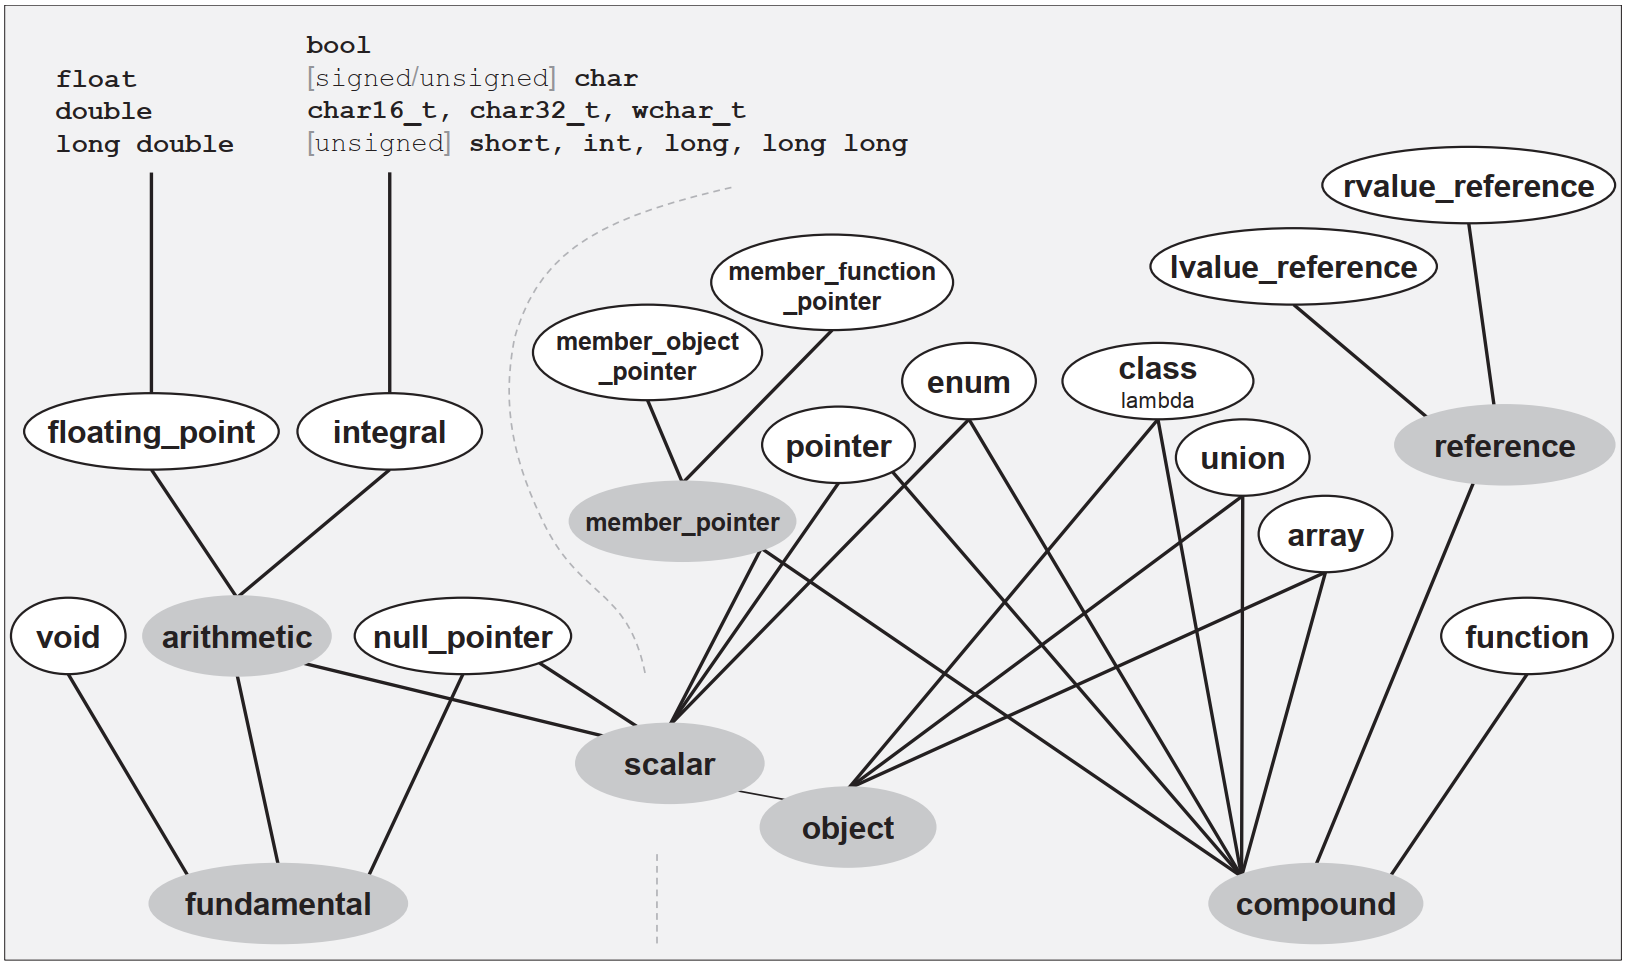
\includegraphics[width=0.65\textwidth]{content/Appendix/D/images/1.png} \\
图D.1. 主要和复合类型类别
\end{center}

\subsubsubsection{D.2.1\hspace{0.2cm}测试主要类型的类别}

本节测试给定类型的主要类型类别。对于给定类型,只有一个主类型类别具有计算结果为true的静态值成员。

\begin{tcolorbox}[colback=webgreen!5!white,colframe=webgreen!75!black]
\hspace*{0.75cm}C++14前,唯一的例外是std::nullptr\_t,对于所有的主类型类别实用程序都产生了false,因为is\_null\_pointer<>不是C++11的一部分。
\end{tcolorbox}

结果与类型是否用const和/或volatile(cv限定)限定无关。

注意,对于类型std::size\_t和std::ptrdiff\_t,当\_integral<>时结果为真。对于类型std::max\_align\_t,这些主要类型类别中哪一个是true是实现的细节(可能是整型、浮点型或类)。语言指定Lambda表达式是类(参见第15.10.6节),将is\_class应用于该类型可得到true。

\begin{table}[H]
	\centering
	\begin{tabular}{|l|l|}
		\hline
		\textbf{特征 }                                                   & \textbf{作用}                                                                                                         \\ \hline
		is\_void\textless{}T\textgreater{}                       & void类型                                                                                                      \\ \hline
		is\_integral\textless{}T \textgreater{}                  & \begin{tabular}[c]{@{}l@{}}整数类型(包括bool, char, char16\_t, char32\_t, wchar\_t)\end{tabular} \\ \hline
		is\_floating\_point\textless{}T \textgreater{}           & 浮点类型(float, double, long double)                                                               \\ \hline
		is\_array\textless{}T \textgreater{}                     & 普通的数组类型(非 std::array类型)                                                                      \\ \hline
		is\_pointer\textless{}T \textgreater{}                   & \begin{tabular}[c]{@{}l@{}}指针类型(包括函数指针,但不包括指向非静态成员的指针)\end{tabular}                                  \\ \hline
		is\_null\_pointer\textless{}T \textgreater{}             & nullptr的类型(C++14)                                                                                  \\ \hline
		is\_member\_object\_pointer\textless{}T \textgreater{}   & 指向非静态数据成员的指针                                                                             \\ \hline
		is\_member\_function\_pointer\textless{}T \textgreater{} & 指向非静态成员函数的指针                                                                         \\ \hline
		is\_lvalue\_reference\textless{}T \textgreater{}         & 左值引用                                                                                           \\ \hline
		is\_rvalue\_reference\textless{}T \textgreater{}         & 右值引用                                                                                           \\ \hline
		is\_enum\textless{}T \textgreater{}                      & 枚举类型                                                                         \\ \hline
		is\_class\textless{}T \textgreater{}                     & class/struct或Lambda类型,但非联合类型                                                               \\ \hline
		is\_union\textless{}T \textgreater{}                     & 联合类型                                                                                                    \\ \hline
		is\_function\textless{}T \textgreater{}                  & 函数类型                                                                                                  \\ \hline
	\end{tabular}
\end{table}

\begin{center}
表D.1. 检查主要类型类别的特征
\end{center}

Lambda表达式的类型是一个类(参见第15.10.6节),将is\_class应用于该类型将得到true。

\textbf{std::is\_void<T>::value}

\begin{itemize}
\item 
如果类型T是(cv限定的)void,则生成true。

\item 
例如:
\begin{lstlisting}[style=styleCXX]
is_void_v<void> // yields true
is_void_v<void const> // yields true
is_void_v<int> // yields false
void f();
is_void_v<decltype(f)> // yields false (f has function type)
is_void_v<decltype(f())> // yields true (return type of f() is void)
\end{lstlisting}

\end{itemize}

\textbf{std::is\_integral<T>::value}

\begin{itemize}
\item 
如果类型T是以下(cv限定的)类型之一,则生成true:

\begin{itemize}
\item [-]
bool

\item [-]
字符类型(char, signed char, unsigned char, char16\_t, char32\_t或wchar\_t)

\item [-]
一个整数类型(short、int、long或long的有符号或无符号;这包括std::size\_t和std::ptrdiff\_t)
\end{itemize}

\end{itemize}

\textbf{std::is\_floating\_point<T>::value}

\begin{itemize}
\item 
若类型T是(cv限定的)float、double或long double则为true
\end{itemize}

\textbf{std::is\_array<T>::value}

\begin{itemize}
\item 
若类型T是一个(cv限定的)数组类型,则生成true。

\item 
由语言规则声明为数组(带或不带长度)的参数可以是指针类型。

\item 
std::array<>不是数组类型,而是类。

\item 
例如:

\begin{lstlisting}[style=styleCXX]
is_array_v<int[]> // yields true
is_array_v<int[5]> // yields true
is_array_v<int*> // yields false

void foo(int a[], int b[5], int* c)
{
	is_array_v<decltype(a)> // yields false (a has type int*)
	is_array_v<decltype(b)> // yields false (b has type int*)
	is_array_v<decltype(c)> // yields false (c has type int*)
}
\end{lstlisting}

\item 
参见第19.8.2节了解实现细节。
\end{itemize}

\textbf{std::is\_pointer<T>::value}

\begin{itemize}
\item 
若类型T是一个(cv限定的)指针,则生成true。包括:
\begin{itemize}

\item[-] 
指向静态/全局(成员)函数的指针

\item[-] 
参数声明为数组(带/不带长度)或函数类型
\end{itemize}

不包括:

\begin{itemize}
\item[-] 
指向成员类型的指针(例如,\&X::m的类型,其中X是类类型,m是非静态成员函数或非静态数据成员)

\item[-] 
nullptr的类型是std::nullptr\_t
\end{itemize}

\item 
例如:

\begin{lstlisting}[style=styleCXX]
is_pointer_v<int> // yields false
is_pointer_v<int*> // yields true
is_pointer_v<int* const> // yields true
is_pointer_v<int*&> // yields false
is_pointer_v<decltype(nullptr)> // yields false

int* foo(int a[5], void(f)())
{
	is_pointer_v<decltype(a)> // yields true (a has type int*)
	is_pointer_v<decltype(f)> // yields true (f has type void(*)())
	is_pointer_v<decltype(foo)> // yields false
	is_pointer_v<decltype(&foo)> // yields true
	is_pointer_v<decltype(foo(a,f))> // yields true (for return type int*)
}
\end{lstlisting}

\item 
参见第19.8.2节了解实现细节。
\end{itemize}

\textbf{std::is\_null\_pointer<T>::value}

\begin{itemize}
\item 
若类型T是(cv限定的)std::nullptr\_t,则是nullptr的类型,则生成true。

\item 
例如:
\begin{lstlisting}[style=styleCXX]
is_null_pointer_v<decltype(nullptr)> // yields true
void* p = nullptr;

is_null_pointer_v<decltype(p)> // yields false (p has not type std::nullptr_t)
\end{lstlisting}

\item 
从C++14开始支持。
\end{itemize}

\textbf{std::is\_member\_object\_pointer<T>::value}

\textbf{std::is\_member\_function\_pointer<T>::value}

\begin{itemize}
\item 
若类型T是一个(cv限定的)指向成员的指针类型(int X::*或对于某些类X的int (X::*)()),则返回true。
\end{itemize}

\textbf{std::is\_lvalue\_reference<T>::value}

\textbf{std::is\_rvalue\_reference<T>::value}

\begin{itemize}
\item 
若类型T分别是(cv限定的)左值或右值引用类型,则生成true。

\item 
例如:
\begin{lstlisting}[style=styleCXX]
is_lvalue_reference_v<int> // yields false
is_lvalue_reference_v<int&> // yields true
is_lvalue_reference_v<int&&> // yields false
is_lvalue_reference_v<void> // yields false
is_rvalue_reference_v<int> // yields false
is_rvalue_reference_v<int&> // yields false
is_rvalue_reference_v<int&&> // yields true
is_rvalue_reference_v<void> // yields false
\end{lstlisting}

\item 
参见第19.8.2节了解实现细节。
\end{itemize}

\textbf{std::is\_enum<T>::value}

\begin{itemize}
\item 
若类型T是(cv限定的)枚举类型,则生成true。这既适用于作用域枚举类型,也适用于非作用域枚举类型。

\item 
参见第19.8.5节了解实现细节。
\end{itemize}

\textbf{std::is\_class<T>::value}

\begin{itemize}
\item 
若类型T是用class或struct声明的(cv限定的)类,包括从实例化类模板中生成的这种类型,则生成真。语言保证Lambda表达式的类型是类(参见15.10.6节)。

\item 
对联合、作用域枚举类型(尽管用enum类声明)、std::nullptr\_t和任何其他类型会产生false。

\item 
例如:
\begin{lstlisting}[style=styleCXX]
is_class_v<int> // yields false
is_class_v<std::string> // yields true
is_class_v<std::string const> // yields true
is_class_v<std::string&> // yields false
auto l1 = []{};
is_class_v<decltype(l1)> // yields true (a lambda is a class object)
\end{lstlisting}

\item 
参见第19.8.4节了解实现细节。
\end{itemize}

\textbf{std::is\_union<T>::value}

\begin{itemize}
\item 
若类型T是一个(cv限定的)联合,包括一个由联合模板的类模板生成的联合,则生成true。
\end{itemize}

\textbf{std::is\_function<T>::value}

\begin{itemize}
\item 
若类型T是一个(cv限定的)函数类型,则生成true。对函数指针类型、Lambda表达式的类型和其他类型产生false。

\item 
根据语言规则声明为函数类型的参数,实际上可以是指针类型。

\item 
例如:
\begin{lstlisting}[style=styleCXX]
void foo(void(f)())
{
	is_function_v<decltype(f)> // yields false (f has type void(*)())
	is_function_v<decltype(foo)> // yields true
	is_function_v<decltype(&foo)> // yields false
	is_function_v<decltype(foo(f))> // yields false (for return type)
}
\end{lstlisting}

\item 
参见第19.8.3节了解实现细节。
\end{itemize}

\subsubsubsection{D.2.2\hspace{0.2cm}复合类型类别的测试}

以下类型可以确定类型是否属于更一般类型类别,该类型类别是一些主要类型类别的联合。复合类型类别不构成严格的划分:一个类型可以属于多个复合类型类别(例如,指针类型既是标量类型又是复合类型)。同样,cv限定符(const和volatile)在对类型进行分类时无关。

\textbf{std::is\_reference<T>::value}

\begin{itemize}
\item 
若类型T是引用类型,则生成true。

\item 
等价于: 
\begin{lstlisting}[style=styleCXX]
is_lvalue_reference_v<T> || is_rvalue_reference_v<T>
\end{lstlisting}

\item 
参见第19.8.2节了解实现细节。
\end{itemize}


\begin{table}[H]
	\centering
	\begin{tabular}{|l|l|}
		\hline
		\textbf{特性}                                          & \textbf{作用}                                                                                                                                                                                     \\ \hline
		is\_reference\textless{}T \textgreater{}       & 左值或右值引用                                                                                                                                                                 \\ \hline
		is\_member\_pointer\textless{}T \textgreater{} & 指向非静态成员的指针                                                                                                                                                                \\ \hline
		is\_arithmetic\textless{}T \textgreater{}      & 整型(包括bool和字符型)或浮点型                                                                                                                            \\ \hline
		is\_fundamental\textless{}T \textgreater{}     & \begin{tabular}[c]{@{}l@{}}void,整型(包括bool和字符),浮点,或std::nullptr\_t\end{tabular}                                                               \\ \hline
		is\_scalar\textless{}T \textgreater{}          & \begin{tabular}[c]{@{}l@{}}整型(包括bool和字符型)、浮点型、枚举型、指针型、成员\\指针型和std::nullptr\_t型\end{tabular}                           \\ \hline
		is\_object\textless{}T \textgreater{}          & 除void、函数或引用外的类型                                                                                                                                              \\ \hline
		is\_compound\textless{}T \textgreater{}        & \begin{tabular}[c]{@{}l@{}}与 is\_fundamental相反\textless{}T \textgreater{}: 数组、枚举、联合、类、函数、\\引用、指针或成员指针\end{tabular} \\ \hline
	\end{tabular}
\end{table}

\begin{center}
表D.2. 检查复合类型类别的特征
\end{center}

\textbf{std::is\_member\_pointer <T>::value}

\begin{itemize}
\item 
若类型T是任何指向成员的类型,则生成true。

\item 
等价于: 
\begin{lstlisting}[style=styleCXX]
is_member_object_pointer_v<T> || is_member_function_pointer_v<T>
\end{lstlisting}
\end{itemize}

\textbf{std::is\_arithmetic<T>::value}

\begin{itemize}
\item 
若类型T是算术类型(bool、字符类型、整数类型或浮点类型),则生成true。

\item 
等价于: 
\begin{lstlisting}[style=styleCXX]
is_integral_v<T> || is_floating_point_v<T>
\end{lstlisting}
\end{itemize}

\textbf{std::is\_fundamental<T>::value}

\begin{itemize}
\item 
若类型T是基本类型(算术类型或void或std::nullptr\_t),则生成true。

\item 
等价于: 
\begin{lstlisting}[style=styleCXX]
is_arithmetic_v<T> || is_void_v<T> || is_null_pointer_v<T>
\end{lstlisting}

\item 
等价于: 
\begin{lstlisting}[style=styleCXX]
!is_compound_v<T>
\end{lstlisting}

\item 
参见第448页19.8.1节中的IsFundaT的实现细节。
\end{itemize}

\textbf{std::is\_scalar<T>::value}

\begin{itemize}
\item 
若类型T是“标量”类型,则生成true。

\item 
等价于:  
\begin{lstlisting}[style=styleCXX]
is_arithmetic_v<T> || is_enum_v<T> || is_pointer_v<T>
|| is_member_pointer_v<T> || is_null_pointer_v<T>
\end{lstlisting}
\end{itemize}

\textbf{std::is\_object < T >::value}

\begin{itemize}
\item 
若类型T描述了对象的类型,则生成true。

\item 
等价于: 
\begin{lstlisting}[style=styleCXX]
is_scalar_v<T> || is_array_v<T> || is_class_v<T> || is_union_v<T>
\end{lstlisting}

\item
等价于: 
\begin{lstlisting}[style=styleCXX]
! (is_function_v<T> || is_reference_v<T> || is_void_v<T>)
\end{lstlisting}
\end{itemize}

\textbf{std::is\_compound <T>::value}

\begin{itemize}
\item 
若类型T是由其他类型组合而成的类型,则生成true。

\item 
等价于: 
\begin{lstlisting}[style=styleCXX]
!is_fundamental_v<T>
\end{lstlisting}

\item
等价于: 
\begin{lstlisting}[style=styleCXX]
is_enum_v<T> || is_array_v<T> || is_class_v<T> || is_union_v<T>
|| is_reference_v<T> || is_pointer_v<T> || is_member_pointer_v<T>
|| is_function_v<T>
\end{lstlisting}
\end{itemize}



